

\tikzset{every picture/.style={line width=0.75pt}} %set default line width to 0.75pt        

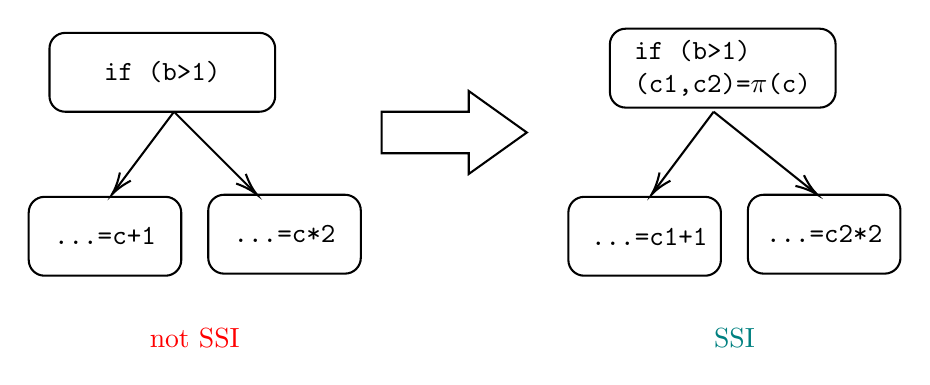
\begin{tikzpicture}[x=0.75pt,y=0.75pt,yscale=-1,xscale=1]
%uncomment if require: \path (0,139.6999969482422); %set diagram left start at 0, and has height of 139.6999969482422

%Rounded Rect [id:dp262243382651531] 
\draw   (10,99.6) .. controls (10,95.4) and (13.4,92) .. (17.6,92) -- (75.9,92) .. controls (80.1,92) and (83.5,95.4) .. (83.5,99.6) -- (83.5,122.4) .. controls (83.5,126.6) and (80.1,130) .. (75.9,130) -- (17.6,130) .. controls (13.4,130) and (10,126.6) .. (10,122.4) -- cycle ;
%Rounded Rect [id:dp4192314773958711] 
\draw   (96.5,98.6) .. controls (96.5,94.4) and (99.9,91) .. (104.1,91) -- (162.4,91) .. controls (166.6,91) and (170,94.4) .. (170,98.6) -- (170,121.4) .. controls (170,125.6) and (166.6,129) .. (162.4,129) -- (104.1,129) .. controls (99.9,129) and (96.5,125.6) .. (96.5,121.4) -- cycle ;
%Rounded Rect [id:dp14874696406611254] 
\draw   (20,20.6) .. controls (20,16.4) and (23.4,13) .. (27.6,13) -- (121.15,13) .. controls (125.35,13) and (128.75,16.4) .. (128.75,20.6) -- (128.75,43.4) .. controls (128.75,47.6) and (125.35,51) .. (121.15,51) -- (27.6,51) .. controls (23.4,51) and (20,47.6) .. (20,43.4) -- cycle ;
%Straight Lines [id:da8036054523449865] 
\draw    (80,51) -- (51.2,89.4) ;
\draw [shift={(50,91)}, rotate = 306.87] [color={rgb, 255:red, 0; green, 0; blue, 0 }  ][line width=0.75]    (10.93,-3.29) .. controls (6.95,-1.4) and (3.31,-0.3) .. (0,0) .. controls (3.31,0.3) and (6.95,1.4) .. (10.93,3.29)   ;

%Straight Lines [id:da9462543361304327] 
\draw    (80,51) -- (118.59,89.59) ;
\draw [shift={(120,91)}, rotate = 225] [color={rgb, 255:red, 0; green, 0; blue, 0 }  ][line width=0.75]    (10.93,-3.29) .. controls (6.95,-1.4) and (3.31,-0.3) .. (0,0) .. controls (3.31,0.3) and (6.95,1.4) .. (10.93,3.29)   ;

%Right Arrow [id:dp5454010361665674] 
\draw   (180,51) -- (222,51) -- (222,41) -- (250,61) -- (222,81) -- (222,71) -- (180,71) -- cycle ;
%Rounded Rect [id:dp804370127764321] 
\draw   (270,99.6) .. controls (270,95.4) and (273.4,92) .. (277.6,92) -- (335.9,92) .. controls (340.1,92) and (343.5,95.4) .. (343.5,99.6) -- (343.5,122.4) .. controls (343.5,126.6) and (340.1,130) .. (335.9,130) -- (277.6,130) .. controls (273.4,130) and (270,126.6) .. (270,122.4) -- cycle ;
%Rounded Rect [id:dp054537017000311994] 
\draw   (356.5,98.6) .. controls (356.5,94.4) and (359.9,91) .. (364.1,91) -- (422.4,91) .. controls (426.6,91) and (430,94.4) .. (430,98.6) -- (430,121.4) .. controls (430,125.6) and (426.6,129) .. (422.4,129) -- (364.1,129) .. controls (359.9,129) and (356.5,125.6) .. (356.5,121.4) -- cycle ;
%Rounded Rect [id:dp9347541053691467] 
\draw   (290,18.6) .. controls (290,14.4) and (293.4,11) .. (297.6,11) -- (391.15,11) .. controls (395.35,11) and (398.75,14.4) .. (398.75,18.6) -- (398.75,41.4) .. controls (398.75,45.6) and (395.35,49) .. (391.15,49) -- (297.6,49) .. controls (293.4,49) and (290,45.6) .. (290,41.4) -- cycle ;
%Straight Lines [id:da09161146890023963] 
\draw    (340,51) -- (311.2,89.4) ;
\draw [shift={(310,91)}, rotate = 306.87] [color={rgb, 255:red, 0; green, 0; blue, 0 }  ][line width=0.75]    (10.93,-3.29) .. controls (6.95,-1.4) and (3.31,-0.3) .. (0,0) .. controls (3.31,0.3) and (6.95,1.4) .. (10.93,3.29)   ;

%Straight Lines [id:da9445970974561072] 
\draw    (340,51) -- (388.44,89.75) ;
\draw [shift={(390,91)}, rotate = 218.66] [color={rgb, 255:red, 0; green, 0; blue, 0 }  ][line width=0.75]    (10.93,-3.29) .. controls (6.95,-1.4) and (3.31,-0.3) .. (0,0) .. controls (3.31,0.3) and (6.95,1.4) .. (10.93,3.29)   ;


% Text Node
\draw (46.75,111) node  [align=left] {{\tt ...=c+1}};
% Text Node
\draw (133.25,110) node  [align=left] {{\tt ...=c*2}};
% Text Node
\draw (74.38,32) node  [align=left] {{\tt if (b>1)}};
% Text Node
\draw (344.38,30) node  [align=left] {{\tt if (b>1)}\\{\tt (c1,c2)=$\pi$(c)}};
% Text Node
\draw (309,111.5) node  [align=left] {{\tt ...=c1+1}};
% Text Node
\draw (393.25,110) node  [align=left] {{\tt ...=c2*2}};

\draw (90,160) node  [align=left] {\textcolor{red}{not SSI}};
\draw (350,160) node  [align=left] {\textcolor{teal}{SSI}};
\end{tikzpicture}
